Puisque le but général de ce travail est d'identifier des groupes sémantiquement cohérents d'entités à partir de leur proximité géométrique, il nous est nécessaire d'évaluer la capacité d'un modèle à plonger les instances d'une même classe dans la même région de l'espace euclidien. On formalise cette exigence en définissant une \textit{tâche de séparabilité}, dont le but est de mesurer si des groupes d'entités appartenant à deux classes différentes sont linéairement séparables.


\subsection{Données}
\label{subsec:kge-data-dbpedia}
Pour entraîner nos modèles, nous avons utilisé la version de DBpédia publiée en octobre 2016, qui était la plus récente jusqu'à récemment, et dont on a exclu l'ontologie DBpédia\footnote{Cette ontologie est accessible au format OWL dans le fichier \texttt{\href{http://downloads.dbpedia.org/2016-10/dbpedia\_2016-10.owl}{dbpedia\_2016-10.owl}}, disponible sur la page de téléchargement de DBpédia} : en particulier, cela signifie qu'aucun triplet \texttt{rdfs:subClassOf} n'est présent dans les données. Le graphe complet contient 3 millions d'entités (insérer le chiffre exacte) et 1.300 relations (idem). Ces entités sont réparties en 589 classes\footnote{On peut trouver la liste actualisée de ces classes à l'adresse : \href{mappings.dbpedia.org/server/ontology/classes/}{https://mappings.dbpedia.org/server/ontology/classes/}}, elle-mêmes distribuées sur sept niveaux de hiérarchie : au niveau 0, on trouve la classe racine \texttt{owl:Thing} dont toutes les entités font partie; au niveau 1, il y a vingt-quatre classes (dont les plus fréquentes sont \dbo{Agent}, \dbo{Place}, \dbo{Agent}), etc. 

L'entraînement se fait avec la librairie OpenKE \cite{openke}. On choisit une dimension de plongement de $d=50$; pour les autres hyperparamètres, on utilise ceux fournis par les auteurs de chaque modèle.

\subsection{Méthodes et variables d'analyse}
\label{subsec:kge-sep-method}

Le principe général est le suivant : pour deux classes $A$ et $B$, on prélève aléatoirement $N$ instances de $A$ et $N$ instances de $B$; on attribue aux instances de $A$ l'étiquette $0$ et à celles de $B$ l'étiquette $1$. Le résultat est un jeu de données $D = \{\mathbf{e_i}, y_i \}_{i=1, \ldots, 2N}$, avec $\bf{e}_i \in \R^d$ le plongement vectoriel de l'entité $e_i$, et $y_i \in \{ 0, 1\}$ l'étiquette associée à $e_i$. 
On sépare $D$ en deux groupes : $D_\textrm{entraînement}$ contenant 75\% des points, et $D_\textrm{test}$ contenant les 25\% restants. On entraîne alors une SVM linéaire sur $D_\textrm{entraînement}$, et on prédit ensuite les étiquettes des entités de $D_\textrm{test}$.
% On entraîne alors une SVM linéaire sur 75\% de ces points, et on prédit ensuite les étiquettes des 25\% restants. 
Les étiquettes comparées peuvent alors êtres prédites aux étiquettes d'origine, selon les mesures usuelles de la classification automatique : précision, rappel, mesure $F1$. 

Pour calculer ces métriques, notons $A_\textrm{pred}$ l'ensemble des entités de $D_\textrm{test}$ qui ont été attribuées à la classe $A$ par le classificateur SVM, et $A_\textrm{vrai}$ les entités de $D_\textrm{test}$ qui appartiennent effectivement à la classe $A$ (notons que le choix de $A$ plutôt que $B$ est arbitraire : remplacer l'un par l'autre revient à échanger précision et rappel).
%Notons $\hat{y}_i$ l'étiquette prédite pour l'entité $e_i$. 
La précision est la proportion d'éléments étiquettés $A$ qui appartiennent réellement à $A$ :
\begin{equation*}
    p = \frac{|A_\textrm{pred} \cap A_\textrm{vrai}|}{|A_\textrm{pred}|}
\end{equation*}
Le rappel est la proportion d'éléments appartenant à $A$ qui ont été correctement étiquettés $A$ :
\begin{equation*}
    r = \frac{|A_\textrm{pred} \cap A_\textrm{vrai}|}{|A_\textrm{vrai}|}
\end{equation*}
La mesure $F_1$ est la moyenne arithmétique de la précision et du rappel :
\begin{equation*}
    F_1 = 2 \times \frac{p \times r}{p + r}
\end{equation*}
Dans nos expériences, on choisit $N=1000$; si une classe possède moins que ces $N$ instances, on utilise toutes les instances de cette classe.

\subsubsection{Variables d'analyse}

La difficulté qu'il y a à séparer une classe $A$ d'une classe $B$ dépend beaucoup de $A$ et de $B$ : intuitivement, il est plus difficile de distinguer un \dbo{College} d'une \dbo{University} qu'un \dbo{Aircraft} d'une \dbo{Person}. De plus, on peut imaginer que la taille de la classe (c'est-à-dire le nombre d'instances qui en font partie) influe aussi sur la difficulté, comme c'est souvent le cas en apprentissage automatique. Nous avons donc mis au point trois métriques pour évaluer la difficulté \textit{a priori} de la tâche de séparation pour toute paire de classe $(A, B)$. La première de ces métriques est la distance lexicale entre les classes, mesurée grâce à des plongements lexicaux; la deuxième est une distance taxonomique entre les classes, basée sur la distance entre les classes dans la taxonomie; la troisième est un indicateur de la fréquence des deux classes dans la base de connaissance.

Ces métriques permettent d'interpréter les résultats de séparabilité obtenus et d'identifier les modèles qui parviennent le mieux à séparer les classes proches ou les classes rares. On les détaille dans les trois paragraphes suivants.


\paragraph{Distance lexicale}

La première de nos métriques est une distance entre les classes, basée sur la proximité sémantique des noms de ces classes. Pour une classe $X$ quelconque, on commence par séparer les mots qui composent son URI : dans DBpédia, la convention de nommage pour les classes est le \textit{CamelCase}, donc l'entité \texttt{SportsTeamMember} est séparée en \texttt{"sports"}, \texttt{"team"} et \texttt{"member"}. On utilise alors des plongements lexicaux pour représenter chacun de ces mots par un vecteur de $\R^d$, et on moyenne ensuite ces vecteurs pour obtenir une représentation vectorielle $\mathbf{X}$ de la classe $X$ de départ. On peut alors définir la distance entre deux classes $A$ et $B$ comme la distance euclidienne entre leurs représentants :
\begin{equation}
d_\text{lex}(A, B) = \| \mathbf{A} - \mathbf{B} \|_2
\end{equation}

Les plongements lexicaux utilisés sont entraînés avec CBOW \cite{mikolov2018advances} sur le Common Crawl, un corpus en anglais comprenant 600 milliards de mots et deux millions de types distincts.

%\footnote{We used word embeddings from \href{https://fasttext.cc/docs/en/english-vectors.html}{https://fasttext.cc/docs/en/english-vectors.html}, trained on Common Crawl \cite{mikolov2018advances}} 

\paragraph{Distance taxonomique}
On introduit également une distance entre les classes basée sur leur distance dans la taxonomie de départ. Puisqu'une taxonomie est un arbre, il existe un unique chemin (non-orienté) de longueur minimale entre n'importe quelle paire de classes $A$ et $B$ dans la taxonomie. En effet, un arbre est un graphe connexe minimal : connexe, donc au moins un chemin existe entre $A$ et $B$; minimal, donc il ne peut exister qu'un chemin, sinon on pourrait supprimer une arête d'un des deux chemins sans perdre la connexité, ce qui contredirait la minimalité du graphe. On note donc $\text{path}(A, B) = \{(A \rightarrow c_1), (c_1 \rightarrow c_2), \ldots, (c_k \rightarrow B)\}$ ce chemin. Pour une arête $e = (c_i \rightarrow c_j)$ donnée, on définit également sa profondeur $\text{depth}(e)$ comme le nombre d'arêtes entre elle et la racine de l'arbre : une arête connectée directement à la racine a une profondeur nulle; une arête connectée à un successeur immédiat de la racine a une profondeur égale à $1$, etc.
On peut alors définir la distance taxonomique comme :
\begin{equation}
    d_\text{tax}(A, B) = \sum_{e \in \text{path}(A, B)} \frac{1}{\displaystyle 2^{\text{depth}(e)}}
\end{equation}
Cette distance taxonomique est la longueur du chemin entre $A$ et $B$, pondérée par la profondeur des arêtes qui composent ce chemin. Le poids d'une arête est $1/2^{\text{depth}(e)}$ et diminue donc avec sa profondeur : en effet, dans une taxonomie, la profondeur d'une arête est un indicateur de la spécificité de l'axiome de subsumption associé à cette arête. Les axiomes associés aux arêtes de profondeur $0$ sont des axiomes très généraux, comme par exemple $\dbo{Place} \sqsubseteq \texttt{owl:Thing}$ («un endroit est une chose») ou $\dbo{Agent} \sqsubseteq \texttt{owl:Thing}$ («un agent est une chose»). À la profondeur $1$, les axiomes sont déjà plus précis – par exemple, $\dbo{Person}\sqsubseteq \dbo{Agent}$ («une personne est un agent»). À des profondeurs plus élevées, les axiomes deviennent très spécifiques, comme par exemple $\dbo{MotorRace} \sqsubseteq \dbo{Race}$ à la profondeur $4$. Aussi, deux classes séparées par une arête de faible profondeur sont sémantiquement plus distantes que deux classes séparées par une arête de profondeur élevée.

Quant au choix d'une décroissance spécifiquement égale à $\frac{1}{2^k}$, il confère à notre distance une propriété intéressante : une classe $A$ est plus proche de ses sous-classes que de n'importe quelle autre classe. Vérifions-le en prenant $A$ une classe de profondeur $d$, et $A'$ une sous-classe de $A$ de profondeur $d' > d$. Alors la distance entre $A$ et $A'$ s'écrit :
\begin{align*}
    d_\text{tax}(A, A') &= \sum_{k = d}^{d'-1} 2^{-k} \\
    &= 2^{-d} \cdot \sum_{k=0}^{d'-d-1} 2^{-k} \\
    &= \frac{1}{2^{d-1}} \left(1 - \frac{1}{2^{d'-d}} \right) 
\end{align*}
Or la distance entre $A$ et sa superclasse immédiate $B$ est :
\begin{align*}
    d_\text{tax}(A, B) &= \frac{1}{2^{d-1}} \\
\end{align*}
Et $d'-d \geq 1$, donc $d_\text{tax}(A, A') < \frac{1}{2^{d-1}} = d_\text{tax}(A, B) \leq d_\text{tax}(A, B')$ pour toute classe $B'$ qui n'est pas sous-classe de $A$. On retrouve bien la propriété énoncée.

\paragraph{Influence de la fréquence}

Une entité $e$ impliquée dans de nombreux triplets sera vue plus souvent pendant la phase d'entraînement, et aura donc un plongement vectoriel plus fiable. Comme ce plongement vectoriel dépend à son tour des plongements des entités et des relations qui sont connectée à $e$, il est possible que les entités appartenant à des classes rares soient impliquées dans des relations rares elles-aussi et connectées à des entités rares; cela produirait des plongements vectoriels moins fiables que la moyenne. Pour vérifier cette hypothèse, on évalue également l'influence de l'effectif des classes (\textit{i.e.} le nombre d'instances qui appartiennent à cette classe) sur les scores de séparabilité. Pour obtenir une mesure synthétique de la fréquence d'une paire de classes $(A, B)$, on utilise la moyenne harmonique des fréquences de $A$ et de $B$. L'utilisation de la moyenne harmonique plutôt que de la moyenne arithmétique usuelle permet de mieux refléter les déséquilibres entre les fréquences de $A$ et de $B$ : si $N_A$ est la fréquence de la classe $A$ et $N_B$ celle de la classe $B$, et que $N_A$ est supérieur à $N_B$ d'un ordre de grandeur, alors la moyenne arithmétique de $N_A$ et $N_B$ a le même ordre de grandeur que $N_A$, et n'indique donc pas que $B$ est rare par rapport à $A$.

\subsection{Résultats}

On évalue six modèles de plongement sur la tâche de séparabilité : TransE, TransH, TransD, DistMult, ComplEx, RDF2Vec. La séparabilité est calculée sur 10 000 paires de classes issues de DBpédia. On donne les scores de séparabilité moyens pour chaque modèle dans le tableau \ref{tab:separability-results}; on aggrège également les résultats pour différentes valeurs de distance lexicale et taxonomique dans la figure \ref{fig:separability-lexical}, et pour différentes fréquences de classes dans la figure \ref{fig:separability-freq}.


\begin{table}[]
    \centering
    \caption[Séparabilité moyenne de différents modèles de plongement]{Précision, rappel et mesure $F1$ moyens pour différents modèles de plongement sur la tâche de séparabilité. En gras, le meilleur résultat pour chaque métrique.}
    \begin{tabular}{|lrrr|}
    \hline 
        Modèle     & Précision  & Rappel & $F1$ \\
        \hline 
        ComplEx   &	90.4	&	89.9	&	89.7 \\
        DistMult  &	92.5	&	91.6	&	91.6 \\
        RDF2Vec   &	\textbf{99.7}	&	\textbf{99.7}	&	\textbf{99.7} \\
        TransE    &	99.4	&	99.1	&	99.2 \\
        TransH    &	93.6	&	92.1	&	92.5 \\
        TransD    &	85.0	&	83.1	&	83.5 \\
        \hline
    \end{tabular}
    \label{tab:separability-results}
\end{table}

\begin{figure}[h]
  \centering
  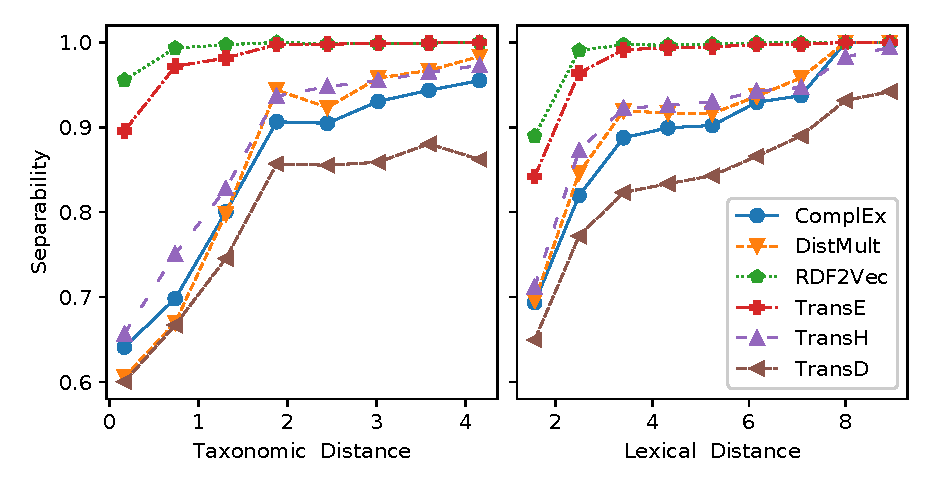
\includegraphics[width=0.8\textwidth]{fig/plot/sep1_dist.eps}
  \caption[Séparabilité moyenne en fonction de la distance entre classes]{Séparabilité moyenne entre deux classes en fonction de leur distance taxonomique (à gauche) et de leur distance lexicale (à droite), pour différents modèles de plongement. }
  \label{fig:separability-lexical}
\end{figure}

\begin{figure}[h]
  \centering
  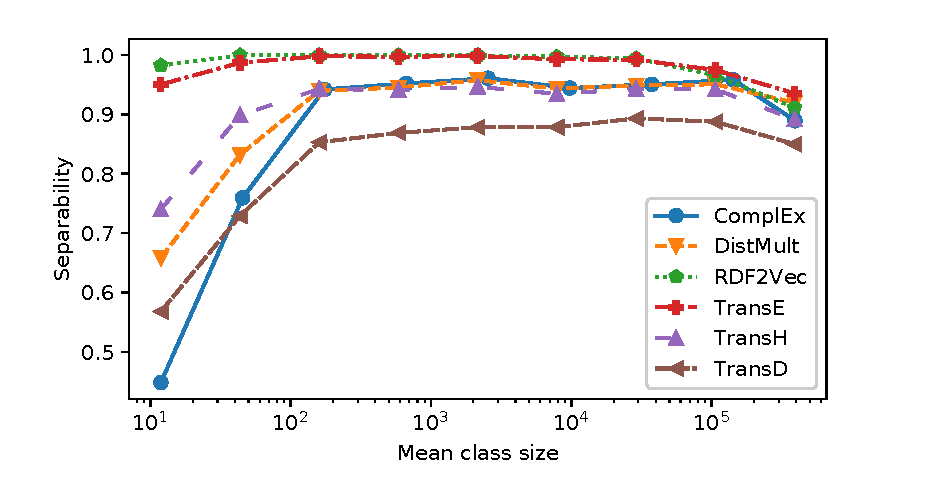
\includegraphics[width=0.8\linewidth]{fig/plot/separability2_type1.eps}
  \caption[Séparabilité moyenne en fonction de la fréquence des classes]{Séparabilité moyenne entre deux classes en fonction de la fréquence de ces classes, pour différents modèles de plongement.}
  \label{fig:separability-freq}
\end{figure}

Comme attendu, le score de séparabilité est dépendant de la distance lexicale et taxonomique entre les classes, et ce pour tous les modèles. Tous les modèles sauf TransD parviennent à séparer correctement les classes distantes (distance lexicale supérieur à 8, ou distance taxonomique supérieure à 3); en revanche, seuls deux modèles parviennent à conserver des scores élevés sur l'essentiel de l'intervalle : RDF2Vec et TransE, avec un avantage net pour RDF2Vec dans les faibles distances. La séparabilité moyenne de ces deux modèles diminue pour les classes très proches (distance taxonomique inférieure à 1, distance lexicale inférieure à 2), mais elle demeure supérieure à 85\%. Tous les autres modèles obtiennent des résultats nettement inférieurs.

Dans la figure \ref{fig:separability-freq}, on observe que les classes rares sont plus difficilement séparables que les classes fréquentes, quoique tous les modèles n'aient pas la même sensibilité à la fréquence : RDF2Vec et TransE n'ont qu'une légère baisse de score pour les classes rares (moins de $10^2$ instances en moyenne), qui peut partiellement être causée par le faible nombre d'échantillons sur lesquels l'algorithme SVM est entraînée. En revanche, les autres modèles ComplEx, DistMult, TransH et TransD y sont très sensibles. Cette sensibilité ne s'explique pas par une corrélation entre les paires rares et les paires proches, puisque les coefficients de Spearman et de Pearson entre les variables de distance et de fréquence sont proches de zéro.

%we observe that rare classes are indeed less separable than more frequent classes, with some variability depending on embedding models. RDF2Vec is once again the best model, with TransE slightly behind. TransH, DistMult and ComplEx have close scores in the size range $[200, 10^5]$, but ComplEx is more sensitive to rare classes than DistMult, which is itself more sensitive than TransH. More surprisingly, we observe that scores also decrease for very frequent classes (mean size above $10^5$ instances) for all embedding models. Both Pearson and Spearman’s correlations between lexical distance and mean class size are close to zero, which rules out the possibility of a bias in the dataset. An explanation is that frequent classes are more likely to be parent of other classes in the dataset (for example, \texttt{dbo:Agent} is the second most frequent class of the dataset, and is a parent of half the classes in the DBpedia ontology), and separating a subclass from its parent is harder than separating sibling or unrelated classes. Finally, we observe a convergence of scores for frequent classes between all models, with TransE achieving the highest score.

En résumé, seuls deux modèles obtiennent une mesure $F1$ moyenne supérieure à 95\% sur notre tâche de séparabilité : RDF2Vec et TransE, avec respectivement 99,7\% et 99,2\%. 
%\label{sec:kge-sep}